%cmd: clear; latex assign1.tex
%cmd: clear; xdvi assign1.dvi



\documentclass{article}
\usepackage[utf8]{inputenc}
\usepackage[english]{babel}
\usepackage{graphicx}

\title{Assignment 1}
\author{Bhishan Poudel}
\date{August 2015}

\begin{document}

\maketitle

\section{Qn.1}

In this question we studied to plot the Bessel functions j0(x) and j1(x).


Pseudo-code to plot jo(x) is:
\begin{verse}
    open a file to store data\\
        if(x<=0)\\
            y = sin(x)/x\\
    close file\\ 
\end{verse}    
Caveat: There is singularity at x = 0, so we used Taylor expansion at points near x = 0.\\
Similar caution was taken to j1(x).\\
The source codes are attaced in the tar file under location:
Homeworks/qn1/

\section{Qn.2}
\subsection{part a}
A beginnig version of source code called 'cnumbers.f90' was provided.
The question asked to prepare a table of different operations of a given
complex number 'z'.
I chose r = 1 and wrote the source code, however,the code works for any other
values of r. We just have to change the value of 1 to any other value in my source
code 'qn1p1.f90'.

\subsection{part b} 

I saved the data of phi vs atan(y/x) and atan2(y,x) in a file called 'qn2WithJumps.dat'
In this code I did not account for the infinity value of tan(pi/2) or other 
integral multiples of pi/2.

I used xmgrace to plot the graph.

In next code I fixed sudden jumps about tangents of integral multiples of pi/2,
by using more points near singularity and precisely avoiding just the singularity
points.

%%%%%%%%% plotting the figure %%%%%%%%%%
\begin{figure}[ht!]
  \caption{Graph with jumps.}
  \centering
    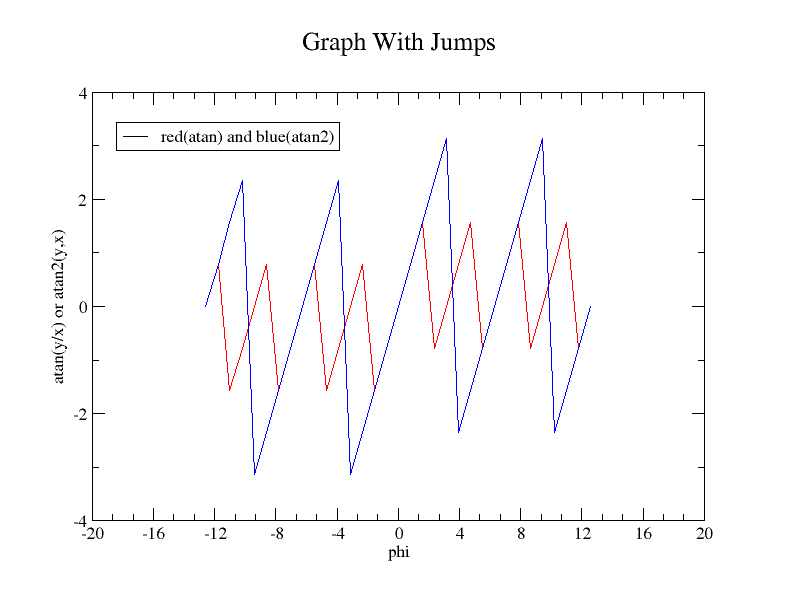
\includegraphics[width=0.5\textwidth]{qn2WithJumps.eps}
\end{figure}

%%%%%%%%%%%%%%%%%%%%%%%%%%%%%%%%%%%%
\begin{figure}[ht!]
  \caption{Graph without jumps}
  \centering
    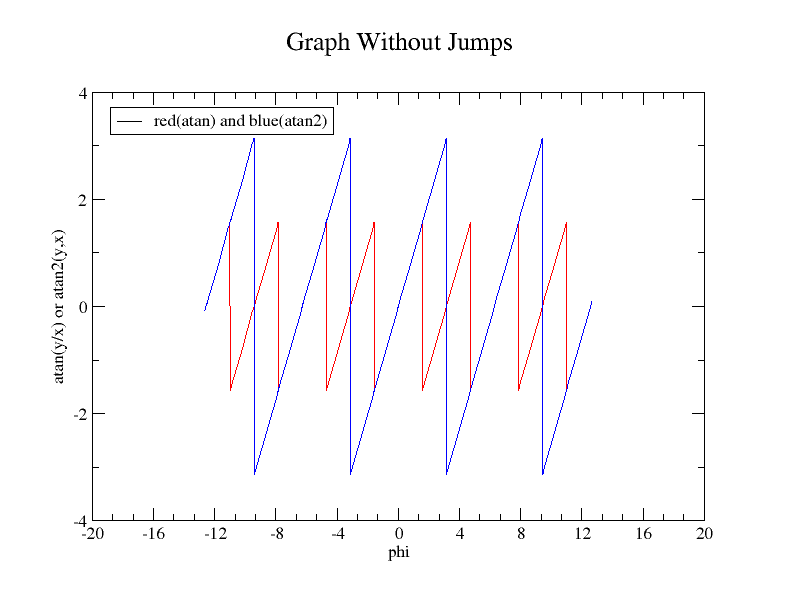
\includegraphics[width=0.5\textwidth]{qn2WithoutJumps.eps}
\end{figure}
%%%%%%%%%%%%%%%%%%%%%%%%%%%%%%%%%%%%%

\subsection{part c}
When I plotted the graph without taking care for infinity effect, it made
some strange jumps. Then i used more points near  a multiples of pi/2 and
avoided being precisely at a integral multiples of pi/2.
The plots are shown above.

\subsection{part d}
I am using SunStudio 12 Fortran Compiler.
It is bright enough to automatically use a complex library routine.

\subsection{part e}
From the descriptions of SunStudio 12 Fortran Libray, I found following:

\subsubsection{ sqrt function}
for a complex number
 
$z = x + iy 
$ 

the square root has also two parts,viz.,real part and imaginary part.

$ z=re^{i \phi} $
    
$ z=r cos(\phi) + r sin(\phi) $

$    \sqrt{z} = \sqrt{r} cos(\phi/2) + \sqrt{r}  sin(\phi/2) $


\subsubsection{ ln function}

$ z = r e^ {i \phi }$

$lnz = ln(r) + i * {\phi} $ 

\subsubsection{ atan(y/x) function}

The function atan(y/x) takes only ONE argument,viz. (y/x).
This is the general arc tangent function.
The function tan(pi/2) gives infinity. So atan(pi/2) gives infinity.
In the plot of atan(y/x) vs phi we get jumps at the 
integral multiples of pi/2 and fixed by taking more points near singularity and
avoiding singular point.


\subsubsection{ atan2(y,x) function}
The function atan2(y,x) takes TWO arguments,viz. y and x.
This is different than arc tangent function.
In our case,

The function tan(pi/2) gives infinity. So atan2(y,x) gives infinity in such cases.
In the plot of atan2(y,x) vs phi we get jumps at the 
integral multiples of pi/2 and fixed by taking more points near singularity and
avoiding singular point.

\section{Qn.3}
In this exercise we examined the power series for the exponential function exp(-x)

\subsection{part a}
The whole source code is given inside /Homeworks/assign1/q3/qn3bad.f90

the pseudo-code to calculate exp(-x) is following:

program expnbad

define variables

write table headers

%%%%%%%%%%%%%%%%%%%%%main pseudo-code 
!use do while loop for different values of x
    
    x = 0.01d0           ! initialize the value of x to be changed later
    
    do while (x < 1000 ) ! loop to get x = 0.1,1.0,10.0,100.0 and 100.0
                       
        x = x*10                  
       
        term = 1.d0   !first term = 1
        
        sum = 1.d0    !sum upto first term
      
        n = 0
        
        factorial = 1.d0 !initialize factorial value
      
        !example 1st iteration: x =1, we will calculate exp(-x) within the error
                    
        do while ((abs(term/sum) > err))
        
            n = n + 1
            
            factorial = factorial *n ! BADWAY
            
            term = term*(-x)/factorial
             
            sum = sum + term
            
        end do
        
        ratio = abs(sum - exp(-x))/sum ! given in the question
             
        write(kwrite,100) x,term,sum,ratio
        
        100 format (3x,F6.1,3(3x,E11.4)) ! formatting the output
        
        ! 3x = 3space, f6.1 = float of width 6, and 3 other scientific values
    
    end do ! end of loop for eg x = 0.1/1.0/etc
%%%%%%%%%%%%%%%%%%%%%%%%%%%%%%%%%%
write the output into a file
%%%%%%%%%%%%%%%%%%%%%%%%%%%%%%%%%%%%%%%%%%%%%%%%%%%%%%%%%%%%%%%%%%%%%%%%
The corrected code fragment for good way is following:

!use do while loop for different values of x 
   
    x = 0.01d0           ! initialize the value of x to be changed later
    
    do while (x < 1000 ) ! loop to get x = 0.1,1.0,10.0,100.0 and 100.0 
                      
        x = x*10                  
       
        term = 1.d0   !first term = 1
        
        sum = 1.d0    !sum upto first term
      
        n = 0
      
        !example 1st iteration: x =1, we will calculate exp(-x) within the error
                    
        do while ((abs(term/sum) > err))
        
            n = n + 1
            
            term = term*(-x)/float(n) 
            
            sum = sum + term
            
        end do
        
        ratio = abs(sum - exp(-x))/sum ! given in the question
             
        write(kwrite,100) x,term,sum,ratio
        
        100 format (3x,F6.1,3(3x,E11.4)) ! formatting the output
        
        ! 3x = 3space, f6.1 = float of width 6, and 3 other scientific values
    
    end do ! end of loop for eg x = 0.1/1.0/etc




\subsection{part b}
The output of bad way is following:

   x       imax          sum           ratio    
   
      0.1   -0.2894E-09    0.9049E+00    0.8796E-04
      
      1.0   -0.7974E-11    0.4201E+00    0.1243E+00
      
     10.0    0.1978E-07   -0.1046E+02   -0.1000E+01
     
    100.0    0.1502E-07    0.1883E+05    0.1000E+01
    
   1000.0   -0.3762E-02    0.6865E+10    0.1000E+01
  
    $The cpu_time =   1.4500000000000006E-004 seconds$

real	0m0.002s

user	0m0.000s

sys	0m0.001s








The output of good way is following:


       x       imax          sum           ratio    

      0.1    0.1389E-08    0.9048E+00    0.2166E-10
      
      1.0    0.2088E-08    0.3679E+00    0.4073E-09
      
     10.0   -0.3867E-12    0.4540E-04    0.4544E-08
     
    100.0    0.1787E+18   -0.2914E+26   -0.1000E+01
    
   1000.0     -Infinity     -Infinity           NaN
    

    $The cpu_time =    3.2000000000000019E-004 seconds$

real	0m0.042s

user	0m0.000s

sys	0m0.002s


\subsection{part b1}
The illustration of underflow of numbers when using bad way and good way is
presented above.

\subsection{part b2}
The table for bad code as well as table for good code was produced.

\subsection{part b3}
I used built in function 'time' in the bash command to find the 
time of compilation. Also i used $'call cpu_time()'$ inside fortran code 
to find the time of compilation.

%%%%%%%%% plotting the figure %%%%%%%%%%
\begin{figure}[ht!]
  \caption{Graph with jumps.}
  \centering
    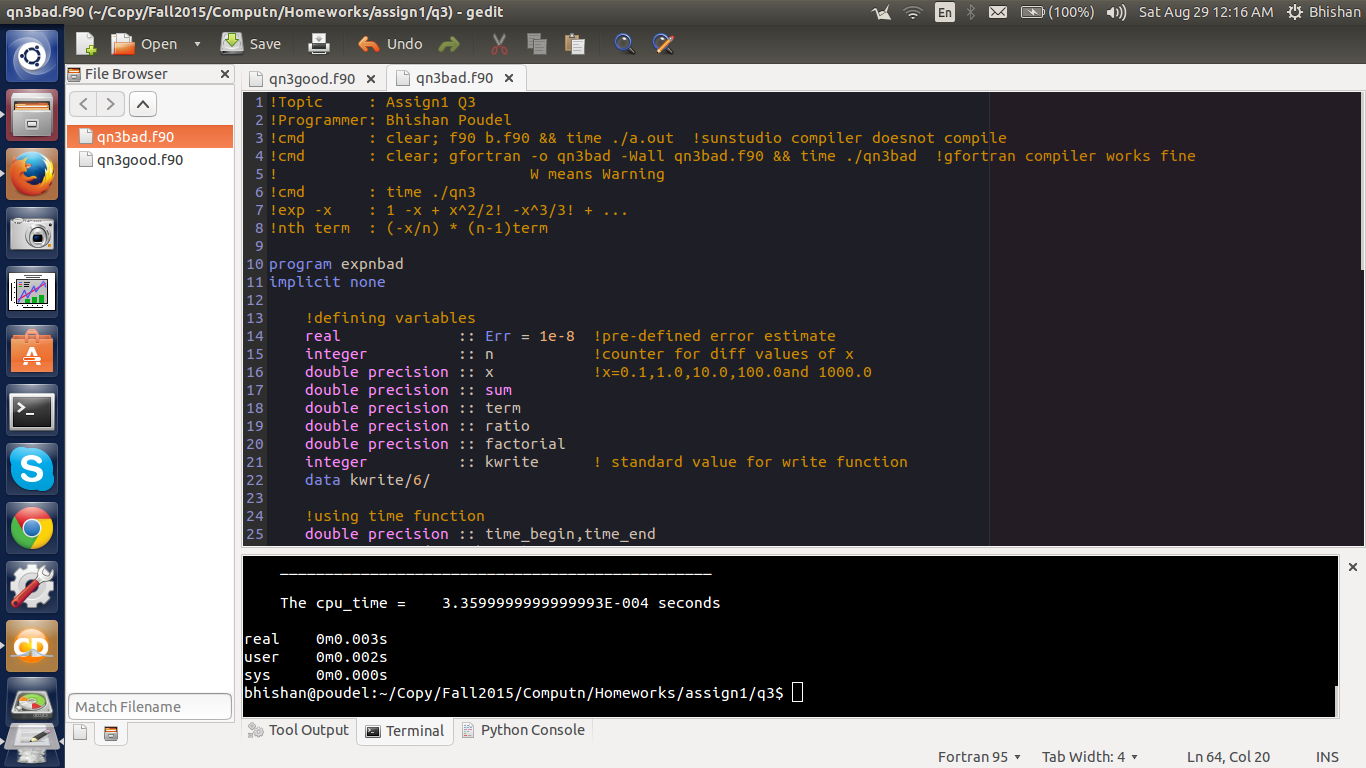
\includegraphics[width=1.5\textwidth]{qn3bad.eps}
\end{figure}

%%%%%%%%%%%%%%%%%%%%%%%%%%%%%%%%%%%%
\begin{figure}[ht!]
  \caption{Graph without jumps}
  \centering
    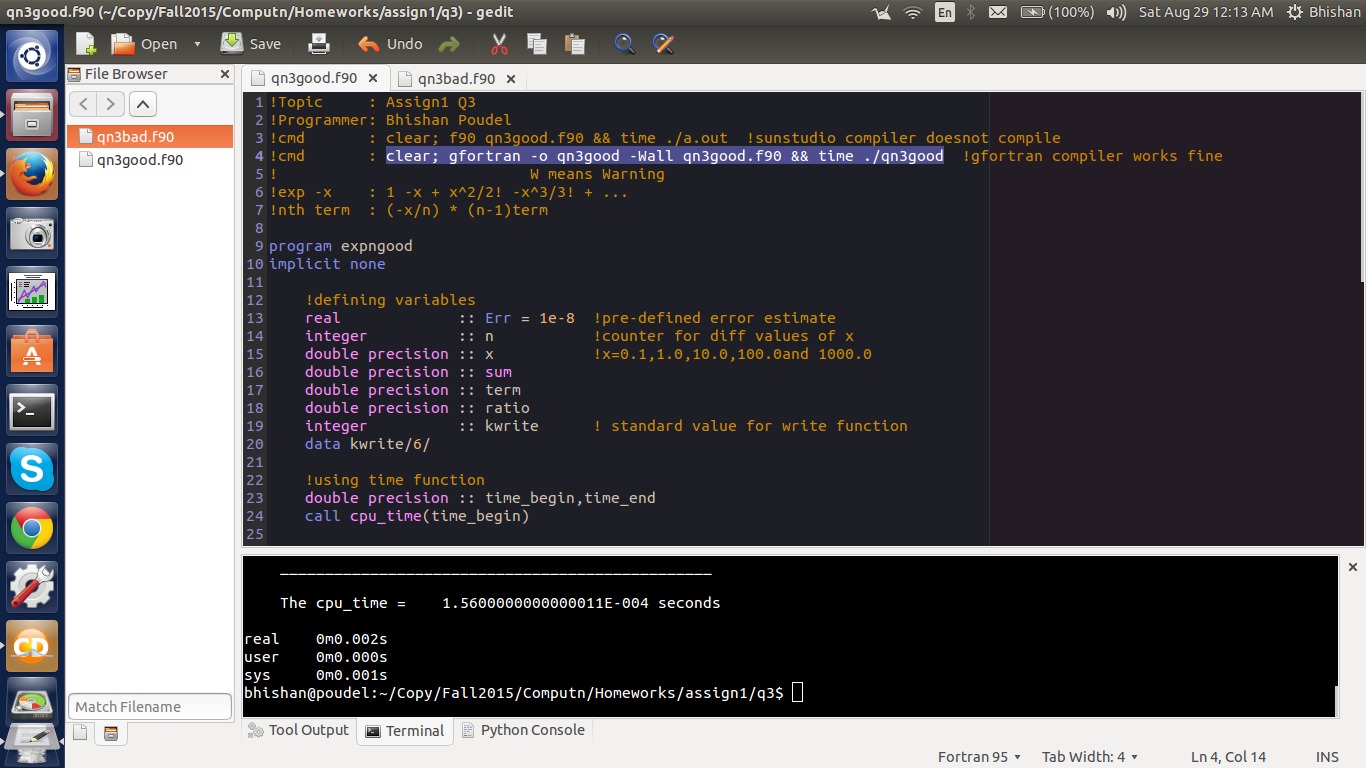
\includegraphics[width=1.5\textwidth]{qn3good.eps}
\end{figure}
%%%%%%%%%%%%%%%%%%%%%%%%%%%%%%%%%%%%%



\end{document}

